\begin{problem}{그림 그리기}{standard input}{standard output}

상수는 $N$행 $M$열의 격자에 $L$가지 색으로 그림을 그린다. $1$행에서 시작해서 $N$행까지, 같은 행에서는 $1$열에서 시작해서 $M$열까지 순서대로 칠하는데, $1$번 색부터 시작해서 $L$번 색까지 순서대로 사용한 뒤 다시 $1$번 색부터 사용한다. $i$번째 행의 높이는 $H_i$이고 $j$번째 열의 너비는 $W_j$이다. 상수는 물감을 낭비하고 싶지 않기 때문에, 그림을 그리기 전에 각 색이 얼마나 필요한지가 궁금해졌다. 상수를 위해 각 색으로 칠할 넓이가 얼마나 되는 지 구해보자.

\InputFile
첫 번째 줄에 $N$, $M$, $L$가 주어진다. ($1 \le N, M, L \le 123,456$)

두 번째 줄에 각 행의 높이를 나타내는 $N$개의 자연수 $H_i$가 공백을 사이에 두고 주어진다. $H_i$의 합은 $10^9$을 넘지 않는다. ($1 \le i \le N$)

세 번째 줄에 각 열의 너비를 나타내는 $M$개의 자연수 $W_j$가 공백을 사이에 두고 주어진다. $W_j$의 합은 $10^9$을 넘지 않는다. ($1 \le j \le M$)

\OutputFile
$L$줄에 걸쳐 $k$번째 줄에 $k$번 색으로 칠할 넓이를 출력한다.

\Example

\begin{example}
\exmp{4 5 3
2 4 3 4
2 4 1 2 5}{63
70
49}%
\end{example}

\Notes

상수가 그릴 그림은 다음처럼 생겼다.

\begin{center}
  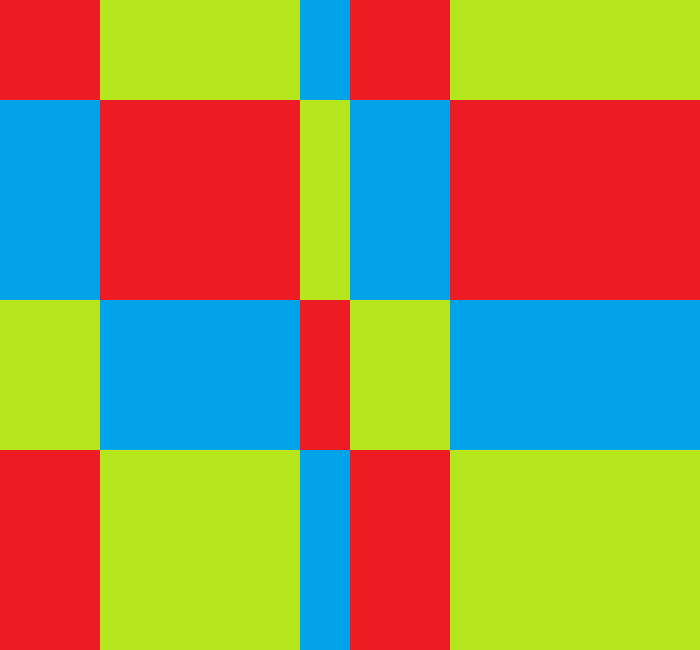
\includegraphics[width=0.5\textwidth]{picture.png}
\end{center}

\end{problem}
